\documentclass[journal]{IEEEtran}
\usepackage{amsmath,amsfonts}
\usepackage{algorithmic}
\usepackage{algorithm}
\usepackage{array}
\usepackage[caption=false,font=normalsize,labelfont=sf,textfont=sf]{subfig}
\usepackage{textcomp}
\usepackage{stfloats}
\usepackage{url}
\usepackage{verbatim}
\usepackage{graphicx}
\usepackage{cite}
\hyphenation{op-tical net-works semi-conduc-tor IEEE-Xplore}
% updated with editorial comments 8/9/2021

\begin{document}
\title{Title}
\author{Wenjin Xu, Chenguang Yang~\IEEEmembership{Fellow,~IEEE,}
    \thanks{This paper was produced by the IEEE Publication Technology Group. They are in Piscataway, NJ.}
    \thanks{Manuscript received April 19, 2021; revised August 16, 2021.}}

% The paper headers
\markboth{Journal of \LaTeX\ Class Files,~Vol.~14, No.~8, August~2021}%
{Shell \MakeLowercase{\textit{et al.}}: A Sample Article Using IEEEtran.cls for IEEE Journals}

% \IEEEpubid{0000--0000/00\$00.00~\copyright~2021 IEEE}
% Remember, if you use this you must call \IEEEpubidadjcol in the second
% column for its text to clear the IEEEpubid mark.

\maketitle

\begin{abstract}
In our daily life, human can accomplish complex tasks with great ease by inspiring and generalizing a set of fundamental skills from the past. Notably, it would be outstanding for the robotic control systems to benefit from such brilliant learning capability. In the last decades, many researchers have paid their massive efforts to investigate the robotic motor control learning problems to provide reasonable decision-making and advanced control methods, such as sliding mode control, adaptive NN control and robust control, etc. In general, it is well known that the robot dynamic is hard to be modeled appropriately with the increasing complexity of manipulator's structure. Due to the excellent approximation capability of NN and fuzzy system, they have been extensively utilized for adaptive control systems to estimate the unknown dynamic of robot at any specific accuracy. Particularly, a notable method which incorporates the fuzzy logic to adaptive NN control has been widely adopted to address the problems of lacking automatic learning capabilities in fuzzy system. By considering the uniform boundedness and state constraints, He~\textit{et al.} proposed an adaptive fuzzy neural network (FNN) control to address the interaction problem of robot. In, a developed FNN control structure is employed to approximate the uncertain dynamic model of a dual-arm robot. Despite much progress achieved in model approximation, several other methodologies have been proposed to ensure the control performance, such as input saturation which can tackle the control problem related to input constraint, finite-time
convergence control.
\end{abstract}

\begin{IEEEkeywords}

\end{IEEEkeywords}

\section{Introduction}
\IEEEPARstart{D}{uring} the past few years, increasing robotic manipulator techniques have been employed into industrial applications and our daily life. One of the most difficult problems in robotic research is how to achieve the human-like working manner in its workspace, such as distinctive capability of skills learning and friendly desirable interaction control. Such abilities are of great importance to enable robots to respond more intelligently and be able to fulfil more complex, dexterous and versatile tasks in various fields such as industrial applications and service areas. 

Nevertheless, a key problem in the aforementioned control schemes which is tough to address is that the neural nodes for NN or the logic rules for fuzzy system are specified beforehand in terms of the expert experiences. Once the desired motion trajectory or working environment is changed, the original controller, unsurprisingly, may result in poor control tracking performance even irreversible consequence. In such case, the FNN controller, which is lack of generation ability from neural biological attribute point of view, needs to be redesigned to deal with the new tasks. Recently, a novel framework named broad learning system, which is developed from random vector functional-link neural networks (RVFLNN), has been proposed and extensively utilized for pattern recognition and classification. By taking the advantages of RVFLNN, BLS can offer acceptable generalization and efficient expansion performance through increasing the neural nodes dynamically. Herein, this inspires us to bring a forward solution which incorporates BLS to improve the generalizing ability of FNN.

As mentioned above, it is innate for humans to adjust the impedance and force of their arms skillfully while interacting with the unknown environments. From a biological point of view, humans can adapt their endpoint impedance of limbs through the central nervous system to achieve compliant interaction. Therefore, it would be crucial and significant to control robot in such way for a variety of social applications such as health care, assembly line and human-robot collaboration. In the literature, significant progress has been made to tackle such related issues. Generally, it is of great importance to establish a desired impedance model for impedance control parameters of which are difficult to choose from in practical. One of the most important parts of impedance control is to determine the desired impedance parameters. Nevertheless, most existing impedance control methods used fixed and manual designed impedance model. In order to improve the performance of compliant interaction under unknown environment, optimization of the impedance model should be taken into consideration. In, a desirable force regulation and tracking performance have been achieved by means of linear quadratic regulator (LQR), which is operated by considering a minimal cost function, to optimize the impedance parameters under a vital precondition of completely known environment dynamics. However, such algorithms seem too conservative to achieve a desired robot-environment interaction since they lack the ability of incorporating the unstructured and dynamic environments. Progress has been made in addressing such problems, and various optimal control schemes in the case of unknown environment have been proposed in literature. It proposed a force sensorless admittance control for robots to tackle with the unknown robot-environment interaction.

The main contributions of this article are listed as follows. \cite{Ju2012}.

1) We propose a learning method based on DMP and FGMM which can not only learn the trajectory from multiple demonstrations but also learn the deviation among them.

2) We present a new LfD method which can demonstrate by single static image, each sample point on the image is encoded by a prior trajectory and FGMM. Skills are then learned through the proposed methods

3) We give a method for generating a priori trajectories of Chinese characters, and design a robot learning framework for learning to write. Experiments were carried out on the LASA dataset and Chinese character images to verify the effectiveness of the method.

\begin{figure*}[!t]
    \centering
    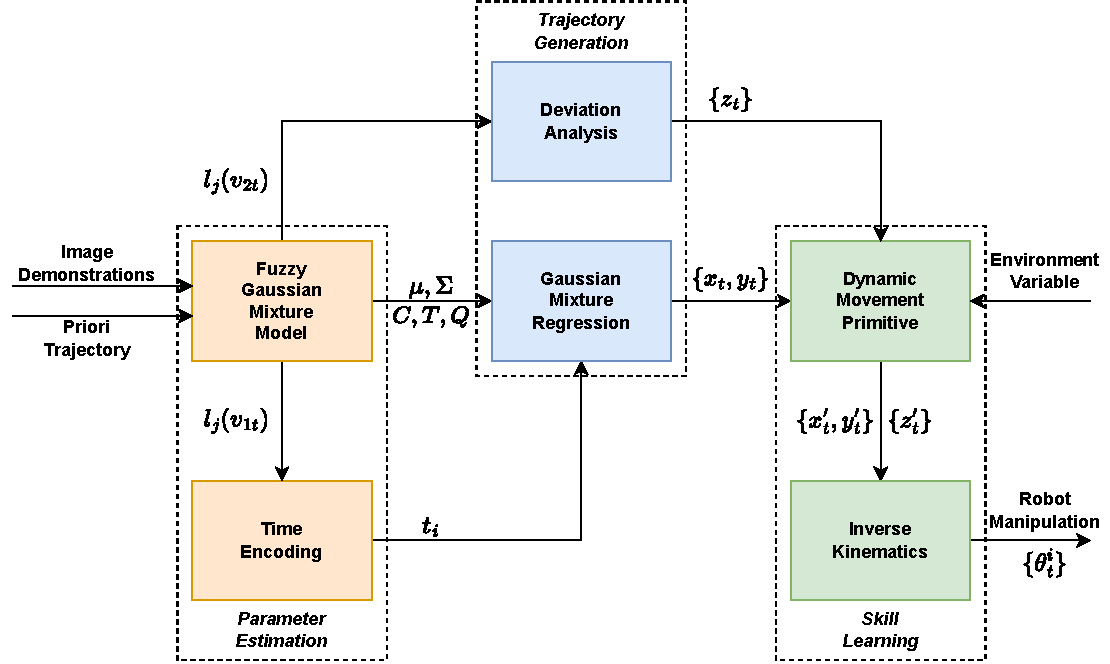
\includegraphics[width=6in]{./fig/fig1.pdf}
    \caption{Block diagram of the proposed system.}
    \label{fig1}
 \end{figure*}
    

\section{Learning the trajectory and deviation \\from multiple demonstrations}

\subsection{Fuzzy Gaussian Mixture Model}

\subsection{Dynamic Motion Primitives}




\section{Learning from static image}


\section{Experiments}
\subsection{Robot writing learning framework}


\section{Conclusion}



\bibliographystyle{IEEEtran}
\bibliography{IEEEabrv,reference.bib}

\end{document}


